\documentclass{notube}
\usepackage{capt-of}


\WP{7c} \WPName{Internet TV in the Social Web}

\delID{7c.2} \delName{Social TV: Sharing of interests and attention data, v.1}
\delNameRunning{Deliverable D7c.1} \delCoordinators{Vicky Buser (BBC)}

\delContributors{Libby Miller (BBC), Dan Brickley (VU)}

\delQualityAssessor{Luca Vignaroli}

\delQualityController{Lyndon Nixon}

\dueContractual{M23}
\dueActual{31-12-10}
\status{0.9}

%\final

\prototype
%\report
%\dissemination

\public
%\consortium

\authorPartner{Vicky Buser (BBC), Libby Miller (BBC),  Dan Brickley (VU)}
\responsibleAuthor{Vicky Buser (BBC)}
\responsibleAuthorPartner{BBC}
\responsibleAuthorEmail{vicky.buser1@bbc.co.uk}
\responsibleAuthorPhone{+44 (787) 6565561}

\summary{
The main objective of this deliverable is to provide an update of the work in workpackage WP7c, `TV and the Social Web'. 

The focus of our Year 1 prototype was on re-using a user's existing activity data from social media sites to generate personal programme recommendations based on the user's interests. The prototype linked the TV to the Web in both directions using the XMPP/Jabber `Buttons' protocol as an API. It also included use of a smartphone as a second screen for controlling the TV, and as a companion device for reading background information about a programme.

During Year 2 we have continued to focus on the value of APIs to TV and on using the XMPP `Buttons' protocol. We also continue to investigate finding ways of filtering interesting video content and bringing it to the user's attention. Given the reported rise in `couch potato multitasking' (the trend for people to use the TV and the Web simultaneously) and the success of the iPad, we also remain interested in the use of second screens for enhancing the TV experience. 

We have been experimenting with the closer integration of online social activity in this year's prototypes, such as programme recommendations based on Twitter trending topics, and real-time interactivity such as voting. We recognise that NoTube is part of the wider convergence of TV and the Web, and we have therefore been monitoring related trends in user behaviour, the increase in Social TV apps, and the arrival of Web-enabled TV. We have also been looking at video on-demand archives, and how recommendations can be used to surface this often hidden content. Another key strand of this year's work has been dedicated to planning user evaluations. 

We show how this workpackage continues to contribute to the value of the NoTube project by combining a focus on developing re-usable APIs for Social TV with finding ways of using Linked Data to enhance the experience of watching TV. We also define some ongoing research issues and ideas for future work.
}

\abstract{
The focus of our Year 1 prototype was on re-using a user's existing activity data from social media sites to generate personal programme recommendations based on the user's interests. The prototype linked the TV to the Web in both directions using the XMPP/Jabber `Buttons' protocol as an API. It also included use of a smartphone as a second screen for controlling the TV, and as a companion device for reading background information about a programme.

During Year 2 we have continued to focus on the value of APIs to TV and on using the XMPP `Buttons' protocol. We also continue to investigate finding ways of filtering interesting video content and bringing it to the user's attention. Given the reported rise in `couch potato multitasking' (the trend for people to use the TV and the Web simultaneously) and the success of the iPad, we also remain interested in the use of second screens for enhancing the TV experience.
}

\keywords{TV, television, set top box, media centre, iphone, ipad, XMPP, jabber, strophe, voting, companion device}

\versionLog{
    \versionLogEntry{\today}{Vicky Buser}{0.9}
}


\begin{document}

\maketitle

%\include{abbreviations}

\chapter{Introduction}

\section{Deliverable Objective}

The aim of this deliverable, D7c.2, is to:
\begin{itemize}
\item{Summarise the work that has been done so far in this workpackage}
\item{Outline current work}
\item{Describe the most recent prototypes}
\item{Set this work in the broader context of Web and TV convergence}
\item{Identify plans for evaluation and future ideas for research}
\item{Show how this workpackage is adding value}
\end{itemize}

\section{Workpackage Objective}

The objective of workpackage WP7c, `TV and the Social Web', is to demonstrate APIs for linking the Social Web with broadcast and on-demand television, using Linked Data from broadcasters, audiences and across the web, to help make social content navigation applications and active TV communities. The idea is to connect people, their friends, their activities, and their televisions in a suitably privacy-preserving way in order to make TV in the future a more enjoyable and interesting experience.

\section{Summary of previous work}

Our initial prototype connected the TV to the Web in both directions using the XMPP `Buttons' protocol. As shown in Figure 1.1, we  were able to show personalised programme recommendations based on a user's existing activity on the Social Web.  The demonstrator also provided linked data about a programme on a second screen. 

\begin{figure}[htbp]
\begin{center}
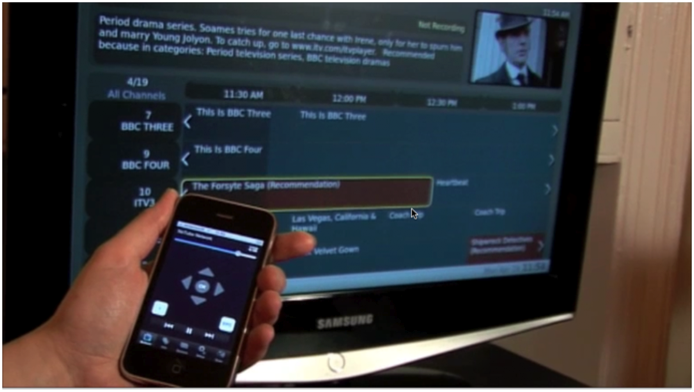
\includegraphics[width=6in]{images/year1.png}
\caption{Year 1 prototype} \label{fig:userview}
\end{center}
\end{figure}


\section{Description of Current Work}

During Year 2 we have been investigating new strategies for helping people decide what to watch, and for making TV a more sociable experience.

Integration of TV and the social web is already happening. People are increasingly using online social networks to talk about TV, nearly all via second screens. This trend started without any specific tools to support it, but increasingly, applications are being built specially - however, they don't need to exist for it to happen. 

Despite this, we still think there are tools that can help people communicate socially about TV - including the infrastructure described below, such as APIs which can improve the integration of the second screen and TV, and other lightweight tools such as targeted autocomplete for TV.

There are also unsolved problems to do with finding video content in large collections, and unmet opportunities around small groups temporarily coming together around TV programmes.

\chapter{Scenarios}

Our scenarios cover a broad range of usecases; from sharing obscure on demand content to participating in popular broadcast events.

\section{How can I find something interesting to watch?}

We are continuing to explore different ways to crack the problem of finding something interesting to watch. Here we take two different approaches each suitable for a different mindset of the person planning to watch TV. 

The first is the person wishing to `lean back' and watch TV, with minimal effort on their part to find something to watch. 

There is evidence to suggest that a high proportion of the conversations in social media are around what people are watching on TV\footnote{For example: a YouGov/Deloitte report published in August 2010 found that 42\% of those UK adults who use the Internet while watching television do so to discuss or comment on the programmes they are watching at the time (http://today.yougov.co.uk/consumer/television-going-social). Similarly, a Twitter survey (conducted by BBC Audience Research) in August 2010 found that 49\% of UK Twitter users in the sample said they used Twitter regularly when watching TV.}. During prime-time scheduling Twitter trending topics are often TV-related, and this Twitter activity can influence what people decide to watch. For example, people reported watching The Eurovision Song Contest on the basis of what was being said about it on Twitter, even though they wouldn't normally have watched it\footnote{\url{http://www.broadstuff.com/archives/1696-Eurovision-songs-sound-better-on-Twitter......html}}. A common way of organising on-demand collections is to allow the user to see what's popular. Social networks allow us to give the user information about the popularity of shows as they are broadcast - and also to see what's popular among their friends, so extending this technique to broadcast TV, and personalising it, with minimal effort on the part of the user.


For the person more willing to engage in `lean forward' effort to find something interesting to watch, we look at the central unsolved problem of finding something to watch from large on-demand video collections. For people willing to put some time into search and browsing, what's popular may be a less satisfactory option than some niche content buried deep in the long tail, and we look at how videos like this might be presented to them.

\section{How can I share what I'm watching with others?}

On the web there cannot be any default assumption of shared context. Unlike TV, many social networks are not geographically constrained and people often have quite diverse networks. Because of this, links are often used to provide some of that context. 

Without a means to refer to the item being watched, the conversation can only go so far. If I'm watching a great documentary on the National Grid I can talk about how great it is using its title, but there the conversation will probably end, unless someone also happens to be watching at the same time. However, if I also give a link then people can find out more about it, perhaps watch it, and perhaps respond to my original comments, sparking a more interesting discussion. 

Providing the means to automatically insert the URL of a programme into users' comments therefore helps to create the structure for more meaningful conversations.

\section{How can I share my emotional reactions to a programme with a wider group?}

Sport, politics, reality shows, comedies and national events can all produce emotional responses in people watching them, and the desire to share some of these feelings is part of the fun of watching these kinds of programmes. The Social Web provides the means to widen out the groups that can participate in this sharing. People need not be physically in the same place, and the groups need not be people you already know. Some broadcasters are already tapping into this experience  - for example Channel 4's game show `The Million Pound Drop' includes an online element that lets users play along live as the show progresses\footnote{\url{http://www.channel4.com/programmes/the-million-pound-drop-live/articles/game}}  that has proved very popular. Reading other people's funny or insightful comments can capture the excitement and emotion of watching TV with others, and encourage individuals to add their own opinions to the conversation. We know this is already happening, so we wanted to take the idea a bit further.

We wanted to explore how social media could be used as a trigger for the formation of ad-hoc interest groups who want to do something specific. The simple example is a group casting real time votes on the popularity of participants of a TV programme, but more complex examples could include collaborative TV annotation or commentary, in small or large groups.  

\section{Business Drivers}

While users remain central to our work, we are not just taking the users' point of view - business concerns are also important considerations:

\begin{itemize}
\item{Many large media organisations have huge archives of video often with metadata describing them. A big problem is: how can people find interesting content in these archives, particularly videos that no-one has watched? Can we (re-)use metadata created with the programme to help them find it? Can this be enhanced with other external sources of metadata? How do people find and share the content? Can social media be used to surface long tail content (that no-one has yet watched)? From a content owner's point of view, there's no point in one person finding something interesting if they can't tell anyone else about it.}
\item{The big advantage of broadcasters is just that: that they have the ability to reach large numbers of people simultaneously. What kinds of applications can encourage people to watch with others? What benefit could these applications bring?}
\item{How can we gather information about interest in the programme over the lifecycle of pre-broadcast, broadcast, on-demand and archive?}
\item{The BBC has a duty to provide for everyone in the UK, not just the relatively small percentage who use social networking while watching TV. Is there a way to use social networks to benefit those large numbers who aren't in social networks?}
\end{itemize}

\chapter{Context: Trends in Web and TV Convergence}

TV and the social web is a very fast moving area. This brief overview of current trends sets our work in context.

\section{Trends in User Behaviour}

The trend for using online social networks to talk about TV continues to increase. For example, YouGov's Social TV trends report\footnote{\url{http://today.yougov.co.uk/consumer/television-going-social}}  found many of the 76\% of 18 to 24-year-olds who browse the Web whilst watching TV want to vote and download information about what they're watching, as well as comment and view reactions to shows in real-time from their friends and family via instant messaging, or through social networking sites.

Research suggests that people often use `second screens' such as a laptop, tablet or mobile phone while watching TV\footnote{\url{http://www.reuters.com/article/idUSTRE62L4UB20100322}}. In the last few months `second screen experiences' specifically designed to complement TV have proliferated  - particularly around live sport events such as the World Cup\footnote{For example \url{https://picklive.com/} and \url{http://mintdigital.com/blog/livepitch}}. This trend has been accelerated by the success of the iPad and its suitability for use in the home for leisure and entertainment purposes\footnote{For example, eMarketer's research has shown that 24\% of iPad owners in the UK use their iPad as their primary entertainment device, and 62\% of iPad owners in a similar study said they had never or rarely taken it out of the house}. Tablets such as the iPad also lend themselves much better than smartphones to being shared among family and friends\footnote{\url{http://blog.nielsen.com/nielsenwire/wp-content/uploads/2010/10/Nielsen-Connected-Devices-Summary-Oct-2010.pdf}}. In addition to their larger screen size, this makes them more suitable for use as a communal TV remote control\footnote{\url{http://www.ericsson.com/news/1440031}}.

\section{Growth in Social TV apps}

We have observed a growing trend, particularly in the US, for second screen services and platforms designed around creating `Social TV' experiences. Several apps and sites (such as Philo, Miso, and GetGlue) have repurposed the check-in concept popularised by Foursquare and adapted it for TV for a shared television watching experience (although it could be argued that people are doing this already by using hashtags for programmes on Twitter).

Other services, such as yap.tv, Starling TV, and Tunerfish are concentrating on integration with Twitter and Facebook. In the UK, BBC's iPlayer catch-up now links with Twitter and Facebook and will feature Microsoft's Windows Live messenger soon. An experimental service, Gawp\footnote{For example: \url{http://gawp.metabroadcast.com/libbymiller}}, has the potential to connect people with similar watching habits.


\section{Web-Connected TVs}

Connecting the TV to the Web has become a focus for manufacturers and makers of set top boxes, with Apple TV, Sony's Google TV, the Boxee Box, and Roku XDS, to name a few, all coming to market. DisplaySearch forecasts that by 2013, 100 million connected TVs will be shipped worldwide, up 546\% from nearly 15 million in 2009\footnote{\url{http://www.displaysearch.com/cps/rde/xchg/displaysearch/hs.xsl/100405_tv_manufacturers_continue_to_breathe_new_life_into_tv_market.asp}}. This development is likely to have an impact on future Social TV scenarios; for example, the potential role of video telephony will be interesting to watch. We also wait to see whether these all-encompassing single-screen solutions threaten to make second screens redundant.

\section{Analysis}

Our position as a research project enables us to take a more user-centric and holistic approach than a purely business-based one, and allows us to identify gaps in the infrastructure and suggest possible future directions.

Here are some key observations driving our work:

\begin{itemize}
\item{APIs to various kinds of TV-like devices and software are proliferating, and this suggests the application equivalent to having many physical remote controls for your TV setup. We know that users don't want this; it also makes things more difficult for manufacturers and application developers. It makes sense to look for the common elements of such an API. Our usecases work is ultimately geared towards being able to feed into such work and propose such an API to a wider community (we hope to do this at the W3C's Web and TV workshop in February 2011).}
\item{The trends suggest that our work on connected second screens is on track with a large portion of the industry. However it is not clear at the moment what second screen applications give the user that existing tools (such as using Twitter or Facebook on a laptop or phone) do not. People started using second screens for TV watching without any of these tools being available. We are therefore attempting to look a step ahead to where future TV APIs might lead.}
\item{There is a strong trend towards the provision of web-connected TVs. However, from a user's point of view, using the Web on the TV is an unfamiliar and relatively uncomfortable proposition, and involves the use of very complicated remote controls or keyboards while watching the TV\footnote{Wow, Sony's Google TV Remote Looks Like A Ten Thousand Button Nightmare: \url{http://techcrunch.com/2010/10/05/google-tv-remote/}}. Further, the user has less control. This screenshot of `dual view' mode for Twitter in GoogleTV\footnote{From \url{http://searchengineland.com/life-with-google-tv-my-first-day-impressions-53471}} shows the majority of the TV screen taken up by the Twitter stream, with the TV content itself confined to the lower right-hand corner. The main experience of watching the baseball game is clearly compromised by this arrangement. It may be that the focus of Web-connected TVs is not the Web per se, but the delivery of video content.} 
\end{itemize}


\begin{figure}[htbp]
\begin{center}
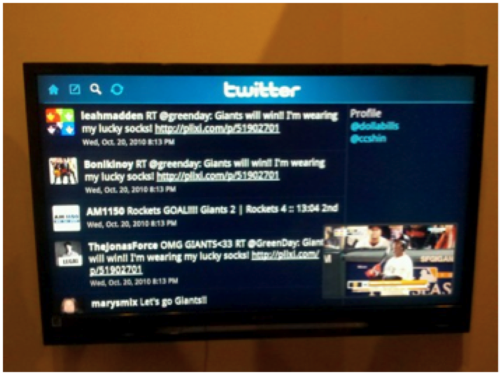
\includegraphics[width=6in]{images/googletv.png}
\caption{Twitter on GoogleTV} \label{fig:google}
\end{center}
\end{figure} 



\chapter{Prototypes}

All the prototypes described below use second screens to allow the user to choose and control comfortably and then, when ready, play on a larger screen. All also use XMPP over http to do the controlling. This technical framework allows us to quickly create two-screen applications in HTML and so speeds development. There is no reason why native XMPP applications could not be used instead.

XMPP is chosen as the messaging prototcol, as before, because of its built-in user-centric `friend-based' security model. We use the Strophe implementation of  XMPP over http and the eJabberd XMPP server. More information about this set up is in this blog post:  \url{http://blog.notu.be/2010/08/06/strophe-and-greasemonkey/}.

More detail about our plans for evaluation of these prototypes is in a later section of this document.

\section{Navigating Large Video Collection Using Linked Data}

This new two-screen prototype is designed to aid serendipitous content discovery and sharing of newly discovered gems. It uses a private research collection of three years' worth of BBC video archive. The goal is to help people find interesting videos to watch. The technique used is to suggest related videos. A relatedness measure is generated based on the number and diversity of the links the programmes have in common.

Our early NoTube experiments with Linked Data programme recommendations were based on automated entity recognition and extraction of terms in programme metadata being matched to relevant DBPedia concepts. The results suggest that using DBpedia alone produces suggestions that are too general, such as `Eastenders is recommended because you like programmes made in the 1980s'. We concluded that there are inherent limitations to such a scattergun approach, which also depends very much on the quality of the source material.  We decided to experiment with using some semi-editorialised data based on Lonclass, a BBC-specific classification system based on Universal Decimal Classification (UDC) codes. This removes some of the sources of potential irrelevancy (the entity recognition) while retaining some of the interesting characteristics of the data (its complexity and diversity) and increasing the relevancy (the TV domain). 

Lonclass provides a rich vocabulary of ready-made programme metadata that is:

\begin{itemize}
\item{Extremely flexible and precise: the structure of the classification allows for detailed multi-concept descriptions of the subject content.}
\item{TV-focused: Since 1964 the BBC has adapted and extended UDC for television content adding specialised subject terms. New terms are created daily for new concepts and subjects to describe scenes, sequences, clips and shots. We propose that the sheer diversity of terms should help with the interestingness of the recommendations.}
\item{Used by professional cataloguers for subject indexing/classification as part of the cataloguing procedure for the BBC's internal TV and radio programme catalogue. Since a human indexer has assigned the specific link between the programme and the term, we might also expect the recommendations to be more accurate as well as more interesting. }
\item{Potentially better than DBPedia for abstract concepts, i.e. for describing the `aboutness' of a programme.}
\end{itemize}

Using the prototype, from any programme the user can follow suggestions for similar programmes based on the number of common Lonclass links between them and the number of different links between them. The idea is to support ``hours of fascinated clicking'' through the programmes archive, similar to the way that following links in Wikipedia articles can take users on surprising and unexpected journeys through the content. 

This prototype is currently restricted to usage within the BBC, the content is UK-specific, and there is generally about a six-week time lag between a programme being broadcast and it being indexed with Lonclass terms. Despite these limitations, it provides us with a useful tool for testing the value to users of navigating a large video collection via programme-to-programme links that are based on granular (and sometimes quirky) concepts.

Our initial experiments gave rich and diverse links between programmes based on their Lonclass categories, with multiple programme pairs linked by more than one category.

You can see a video of the prototype in action:  \url{http://www.flickr.com/photos/nicecupoftea/4945125947/}.

\begin{figure}[htbp]
\begin{center}
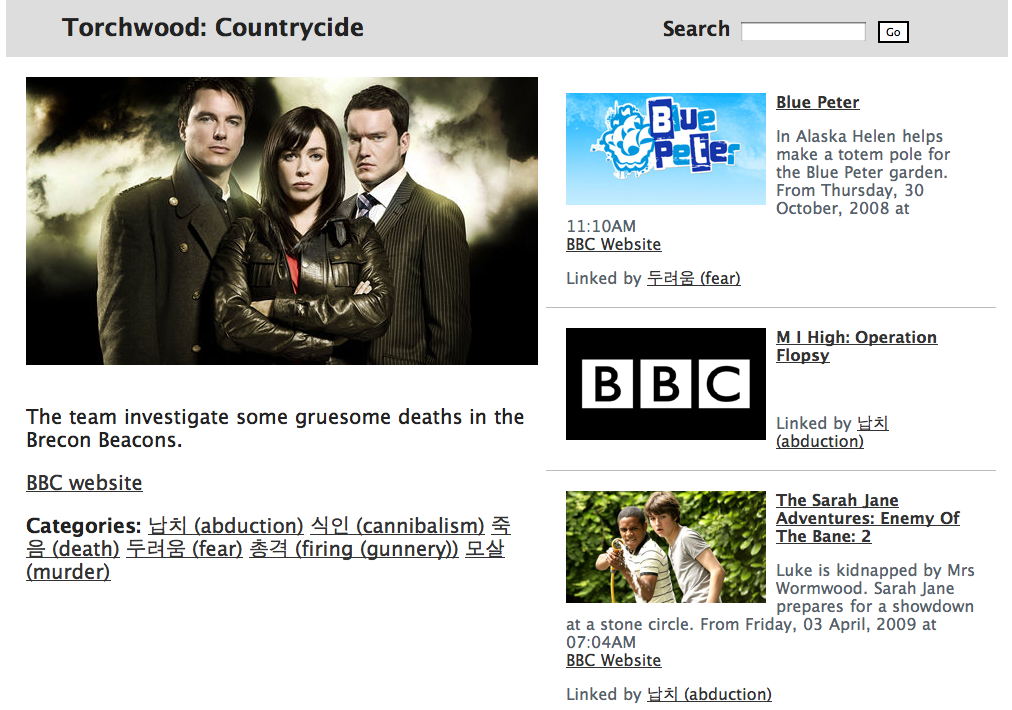
\includegraphics[width=6in]{images/countrycide.png}
\caption{Prototype 1 Screenshot: Korean version} \label{fig:prototype1}
\end{center}
\end{figure}


\section{Interactive Voting}

The second prototype is an application that allows the end user to join an ad-hoc group associated with a broadcast event and get near-immediate feedback on what others are voting for. This initial version is primed with the participants of a political panel broadcast programme in the UK that is popular on Twitter. The user can vote each participant up or down. The goal is to provide a companion to the social network chatter but in a more structured and visual form.


The prototype uses the Twitter API to enable the user to login and then spawns an anonymous XMPP user that connects to a backend vote aggregator. Votes are sent as XMPP messages, aggregated and returned as presence messages for display back to the user. An administration interface allows the addition and deletion of options and enables setting of a hashtag for filtering Twitter messages that the application users see.

\begin{figure}[htbp]
\begin{center}
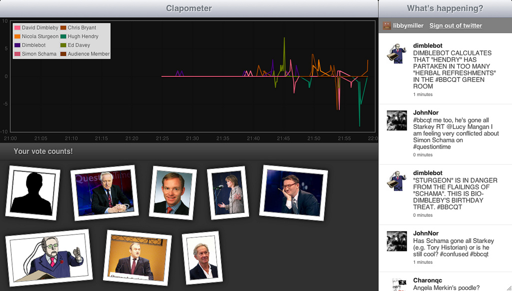
\includegraphics[width=6in]{images/votatron.png}
\caption{Prototype 2 Screenshot: Interactive Voting} \label{fig:prototype2}
\end{center}
\end{figure}

Special thanks to Project Baird and Mo McRoberts for helping design and implement the user interface for his prototype.


\section{Social Extensions to Initial MythTV Prototype}

This prototype is an iPad version of our initial two-screen MythTV prototype incorporating a basic Twitter client and showing social recommendations (initially for broadcast content, but it could also be used retrospectively for on-demand content). It uses levels of Twitter activity around a programme as a source of freely available recommendation data for suggesting items to watch based on trending information. It's a work in progress.

There are several parts to the prototype: 

\begin{itemize}
\item{Showing which programmes are being tweeted about the most as `hot spots' on the EPG, capturing the zeitgeist to suggest programmes of interest.}
\item{Displaying what the user's friends on Twitter are saying about a particular programme.}
\item{Automatically inserting the URL for the programme into the user's tweet.}
\item{Showing on-demand programmes related to those currently showing.}
\item{Showing other programmes that a friend has been tweeting about and make it selectable to watch on-demand.}
\end{itemize}

\begin{figure}[htbp]
\begin{center}
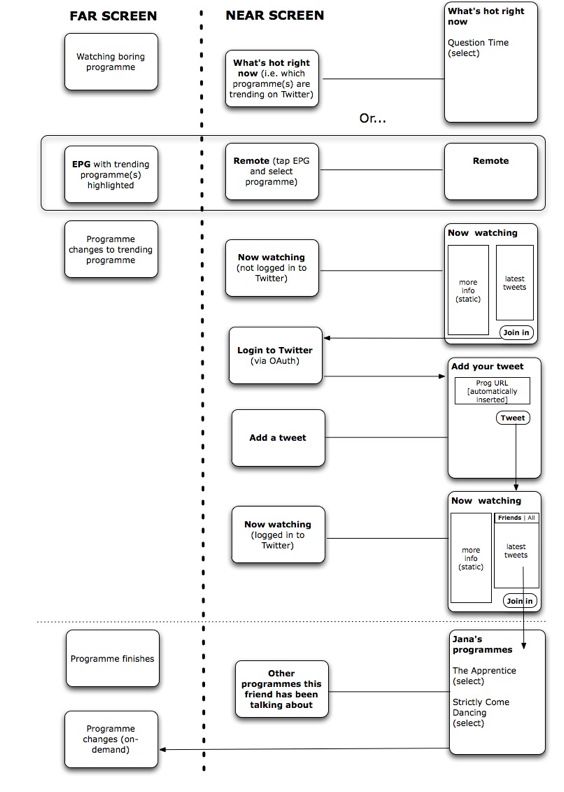
\includegraphics[width=6in]{images/p3arch.png}
\caption{Prototype 3 Architecture} \label{fig:arch}
\end{center}
\end{figure}


\begin{figure}[htbp]
\begin{center}
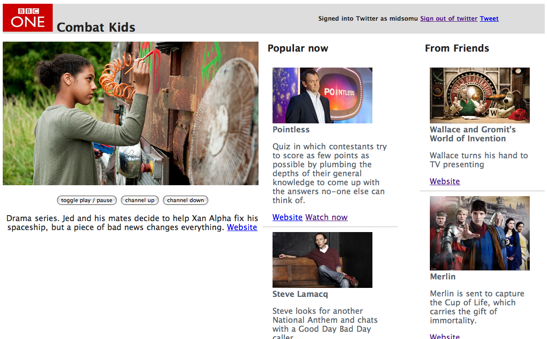
\includegraphics[width=6in]{images/prototype3.png}
\caption{Prototype 3 Screenshot} \label{fig:prototype3}
\end{center}
\end{figure}


\chapter{Infrastructural Work}

To support the prototypes we have continued work on the Open API to TV (`Buttons') and associated services.

\section{Open API to TV}

To avoid the application equivalent of having a different physical remote for each device, the idea of `Buttons' is to create an Open API usable for many different TV applications.  This is the difference between our approach and the various remote control applications available for Boxee, Vimeo, YouTube, TIVO, Apple TV and the Android Google TV remote. The API is the important part, not the specific application of it. 

The API is two-way, including the usual control commands (Play, Pause, etc), additional web-based video commands (Load Page) and also specific responses (Now Playing: at least basic metadata, plus a URL (see TVDNS section below).

\section{CRID Resolver}

This service provides a means of linking from broadcast TV to a webpage describing the programme. The social web is about linking - linking is the usual way of talking about things on the Web. If you can't refer to something by URL, you can't share it.  Although the BBC provides resolvable URLs for each of its programmes, these are not broadcast along with the content, so there is nothing explicitly connecting the URL and the programme being broadcast. Other pieces of information are sent, however, and we can use these to determine the /programmes URL using a resolver.

TVDNS builds on RadioDNS, and allows the use of the DNS system together with some pieces of information that already get sent with the DVB Stream to tell a DNS-capable device that a resolvable URL is a associated with a piece of content. Our implementation is detailed in this blog post: \url{http://blog.notu.be/2010/08/26/connecting-broadcast-tv-and-the-web-using-a-resolver/}. Part of it (CRID  to URL resolution) is used in the third prototype (Social Extensions to MythTV), in order to select appropriate information to display; it also adds the URL of a programme to the tweetbox in that prototype.

\section{EPG Autocompleter}

For less connected devices, we can still make it easier for people to link to programmes by using a filtered autocompleter. This could be used in a tweet box to help people talk about what they are watching. More about the implementation is in this blog post:  \url{http://blog.notu.be/2010/11/22/epg_autocompleter/}.


\chapter{Evaluation plans}

We have highlighted three main areas for user testing that relate to our prototypes. For each of these we have identified a hypothesis and begun designing a test. The tests will be carried out in the first quarter of 2011.

\section{Navigating On-Demand Content Using Interesting Links}

Here we want to test the value of using graph-based `interestingness measures' in a practical experiment to see if this specific application of it produces the expected behaviour - i.e. people carry on clicking through a large video collection by following interesting links.

We plan to conduct a test asking users to browse the first prototype (Navigating Large Video Collection Using Linked Data) whilst adding programmes of interest to a playlist. We will then measure the time spent on this activity and the length and diversity of the playlists compared with measures of the size of the database. We want to see whether the Lonclass-based links have kept people clicking, and enabled individuals to follow their own particular interests.

\section{Using Explanations to Test Linked Data Recommendations}

Research shows that accompanying recommendations with explanations helps users to make more accurate decisions, improves user acceptance of recommendations, and increases trust. A survey of users of one movie recommender study showed that 86\% of those surveyed wanted an explanation feature added to the site (Herlocker et al, 2000\footnote{\url{http://www.grouplens.org/papers/pdf/explain-CSCW.pdf}}). Similarly, users who understand why an item is being recommended reported a higher degree of confidence, liking and understanding (Sinha 2002)\footnote{\url{http://portal.acm.org/citation.cfm?doid=506443.506619}}.

Presenting the pathways through the graphs allows the user to see the connection that led to a recommendation being made. This gives the user a more interesting story than the `black box' explanations of collaborative filtering techniques. Typically such explanations would be like `People who watched this programme also watched these other programmes'. Using graph-based recommendations allows us to say why they are similar: `More programmes about aliens and time travel'. 

We also assume that different types of connections will trigger different levels of interestingness in the explanations, resulting in different levels of user satisfaction. For example, links based on subject may be generally more or less interesting than links based on people (such as actors, directors, authors or presenters).

We plan to test this by randomising the types of recommendations shown to each user (e.g. recommendations based on personal interests compared with content-based recommendations), and showing the associated explanations. We will ask users to complete a questionnaire indicating their satisfaction with each recommendation. We will also conduct lab-based tests for more in-depth verbal feedback to explore which aspects of the explanation made a recommendation interesting to the user, or not.

\section{Second Screens}

Our hypothesis is that, in some contexts, using a second screen to show Web-based information about a programme creates a better user experience than integrating the information with the TV screen, because it:

\begin{itemize}
\item{Doesn't take the user away from main viewing experience} 
\item{Doesn't clutter the TV screen with graphics/widgets}
\item{Is easier for reading and entering text}
\item{Allows for the potential for personalised interfaces}
\end{itemize}

We plan to take the simplest possible scenario (for example: ``show me more about the programme'') and implement it both as widget on a TV and as a simple two-screen prototype, and then conduct lab-based tests to compare users' reactions to the different experiences. In addition to this we are collaborating with our colleagues at VU University to run a student assignment early next year to learn more about how the usability of second screens can be improved to create a more elegant experience.

\chapter{Collaborations}

The goal of WP7c, like the other usecase workpackages, is to help guide the work of the technical workpackages. It has become clear that WP7c requirements differ somewhat from those of WP7a and WP7b, mostly because several years ago the BBC took the decision to make a large amount of metadata public as part of the /programmes project. This means that the conversion of production metadata to make it usable for the usecases has not been necessary as this is already taking place within the BBC in production.

In addition because of our emphasis on rapid prototyping, we have developed and used some sevices that have not yet been incorporated into the general architecture. However our experiences of using them should provide useful within the project in the future.

Nevertheless we have collaborated in multiple ways within the project and outside it, and have specific plans to continue to do so.

\section{User Experience and Evaluation Planning}

BBC (Vicky Buser) and VU (Lora Aroyo) have continued to pursue our common interest in user experience with colleagues, participating in weekly phone calls to discuss user interfaces in the demos, usability issues, and approaches to user evaluations and studies. 

\section{CRID resolver}

BBC (Libby Miller) have been working with Project Baird (Mo McRoberts) on creating a functioning implmentation of TVDNS, which takes data from DVB and looks up a URL using that information. We provided the URL resolver for BBC programmes.

\section{SKOS and UDC}

VU (Dan Brickley) and BBC have had initial discussions with Aida Slavic, UDC Editor in Chief, and Fran Alexander, Taxonomy Manager at the BBC, on how to modernise of subject classification systems, specifically the UDC and BBC's derivative, Lonclass. 

\section{Korean Wordnet (Korlex) version of archive browser}

VU (Véronique Malaise, Ronald Siebes), KT (Teresa Sanghee Kim), and the BBC collaborated to translate programme categories created by the BBC to Korean, via the two step procedure of Lonclass to English Wordnet and then accessing the existing Korlex mapping from English to Korean Wordnet.

\section{Recommendations formats and interfaces}

BBC, Pronetics (Michele Minno) and VU (Balthasar Schopman) on specifying formats for recommendations to be shared between different services, and on an interface to the Beancounter.

\section{iPhone and Strophe development}

VU (Dan Brickley) and BBC (Libby Miller) have been collaborating on the XMPP work both in iPhone application development and HTML-based application infrustructure.

\section{Data Provision}

BBC has provided metadata to Ontotext and VU, to the former for use with Lupedia, and to the latter for data mining Linked Data patterns.

\section{Service Use}

The new version of the MythTV prototype uses services provided by VU (enhancement of BBC content).

\section{Brainstorming and Documentation}

We have shared techniques for brainstorming and documentation (such as card sorting and sketching) with project partners during face-to-face meetings, to bring about improvements to the usability of the project website amongst other things. We hold daily informal IRC chats with collaborators inside and outside the project.


\section{Future Collaborations}

\subsection{Evaluation}

We will fulfil our evalution plans, BBC working with VU doing user testing with students from VU.

\subsection{Different types of recommendations}

Pronetics, BBC and VU intend to work together to show how recommendations might go from cold-start (Linked data-based) to personalised (using Beancounter and social network data) over the same dataset. 

\subsection{Semantic Annotation using Lonclass and DBpedia}

We intend to experiment with Lupedia services to see how Lonclass and DBPedia compare for accuracy and usefulness to the end user.

\subsection{DBpedia / Geonames mappings for Lonclass}

BBC and VU will continue to work on mappings from Lonclass to other vocabularies, with the goal of integrating Lonclass into the Linked Data cloud.


\chapter{How This Workpackage is Adding Value}

\section{By focusing on open, re-usable APIs}

We have created some of the infrastructure for supporting Social TV APIs for effective social engagement with TV, in particular by disambiguating specific programme episodes resolvable via unique IDs. Having this infrastructure in place allows for the development of prototypes that illustrate the use of APIs to TV to support the social elements of both TV and the Web. Making such APIs available for re-use by others is part of the legacy of the NoTube project.

\section{By demonstrating ways in which Linked Data can enhance the TV experience}

Based on our observations of some of the current problems people encounter when watching TV (including too much choice and the difficulty of referring to the specific episode that is being discussed), we continue to investigate ways of using Linked Data to help improve this experience. So far, potential benefits of using Linked Data include the ability to have recommendations and related information `pushed' to end users in a convenient and unobtrusive manner. The serendipitous nature of Linked Data is also potentially very useful in supporting more active discovery of TV programmes that are new and interesting to an individual. The results of our user evaluations may provide evidence of the use of Linked Data to enhance the TV experience for viewers. 

\section{By showing what can be done}

We believe it is beneficial to talk about our results in public as we go along where possible: in doing so we have found a talented and helpful collaborator in Mo McRoberts of Project Baird, and we have been able to gather ideas and interest from inside and outside the project. The techniques we have used - particularly storyboarding, blogging and creating prototypes have been effective communication tools in this fast-moving area.


\chapter{Research Issues and Observations}



\section{Graph Analysis}

In prototype 1 (Navigating Large Video Collection Using Linked Data) we observed that browsing interest is higher when more than one category links two programmes, or when a programme is linked to others by more than one category. We term these two features respectively `pairwise connectedness' and `fanning': browsing interest appears to be higher if pairwise connectedness and fanning are both high. If they are both equal to 1, this is the same as a search for the single category and puts the user in a `rathole' of very similar content, especially given the fine distinctions made in this particular dataset. High pairwise connectedness and fanning mean that there are multiple options for the user to browse.

In preparation for evaluation and for a Korean version of this demonstrator, we started to search for subsets of the data which retain high connectedness and fanning. This turns out to be a complicated task, but an interesting one, because once this data is denormalised it looks very much like a table of triples:

\begin{verbatim}
programme1 - category - programme2
\end{verbatim}

so that we can think of the set of connections between programmes and Lonclass as being a labeled graph, albeit strictly speaking not a directed one (though it can be interpreted as a directed graph). This suggests that investigation into `interestingness' might be extended into RDF graphs in general, and in particular, once we have a measure of it, we should be able to tell if the addition of another graph - for example a set of preferences or an activity stream - is likely to increase interest or not. We intend to look more closely into graph theory for any other features of graphs that can help us characterise their interestingness.

\section{Privacy and Public Data}

Throughout this workpackage we have been mindful of privacy implications, as part of the project's overall goal to `put the user back in the driving seat'. 

In prototype 3 (Social extensions of Initial MythTV Prototype) integrating social influences using publically available Twitter data is one option for eliminating some of the privacy issues around the aggregation and sharing of personal data that we identified in our last deliverable. It's instructive that this is the way in which people seem to be choosing to share their TV consumption data in general, rather than using activity-based aggregators. Whilst there is plenty of evidence of people explicitly talking about programmes, we have found less evidence of people using tools that automate sharing, for all the reasons we discussed before (such as anxieties around indiscriminate disclosure of personal data and perceived high privacy of TV-related activity data).

In prototype 2 (Interactive Voting) the Twitter login isn't strictly required, but is there because the goal is to enhance existing users' use of the social network during the programme, not to replace it. A new anonymous login is spawned each time the user refreshes the page, and no information about the user (such as friends) is kept by the application. Using XMPP we can help people communicate without them needing to have persistent logins. The other interesting issue from a privacy point of view with this prototype has to do with using second screens for social networking. In most cases, it's my social network but our TV, so displaying personal social network comments on the TV screen, as well as being a usability nightmare, is also a privacy problem.

\section{Limiting the Search Space}

A recurring research question is ``how best can we limit the search space to make entity recognition successful?'' This applies to both the Twitter search space (identification of programmes based on short pieces of text) and the related programmes search space (identification of categories based on metadata). These APIs are provided respectively by a BBC team and by Ontotext, so we will just highlight a few items of interest here:

\begin{itemize}
\item{The Twitter search space is limited by time (what's on now) and using specific structured metadata (the names of the participants in a programme, the title of the programme) to improve matching}
\item{The hypothesis in the category matching is that a smaller, TV-related dataset (Lonclass) will produce better results for this purpose than DBPedia / Wikipedia. This needs to be tested.}
\end{itemize}

\section{Evaluation Challenges}

We approach our evaluation work with the observation that getting accurate feedback from users about the quality of programme recommendations is challenging for several reasons. These include the need to for users to try out some new programmes, which might at first seem rather too obscure or too far removed from their traditional choices. Ideally, users would also need to give reflective and retrospective thought to the question of whether a programme recommendation really was `relevant' or `useful', which is difficult to do without actually watching the programme itself.


\chapter{Future Research Ideas}

We have adjusted the work plan in line with the workpackage's position within the wider context of integration of the Social Web with TV, which is accelerating around us.

We are interested in exploring scenarios that involve the use of multiple second screens with TV. For example, a group of friends watching a TV programme, each with their own second screen device, or using a communal second screen such as a touch-table. 

Example scenarios might include:

\begin{figure}[htbp]
\begin{center}
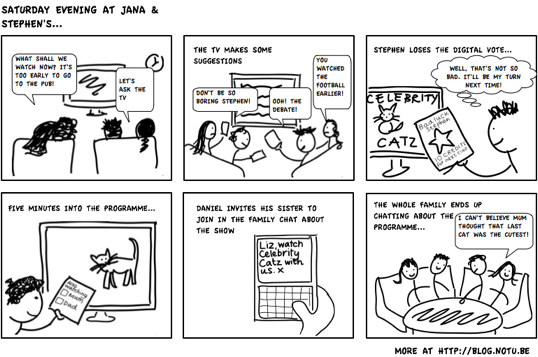
\includegraphics[width=6in]{images/postcard1.png}
\caption{A Possible Scenario} \label{fig:postcard1}
\end{center}
\end{figure}

Another possible focus of work will be around creating useful, rich, link-centred data to specific points in a video. In prototype 2 (`Interactive Voting') in principle any kinds of message could be sent. In some ways the administration of the application is more fun than voting with it, and so potential applications include collaborative annotation of video for example. Links created in such a way could support more meaningful online conversations around, for example, news stories, controversial sporting moments, political debates, or plot lines in dramas. For example:

\begin{figure}[htbp]
\begin{center}
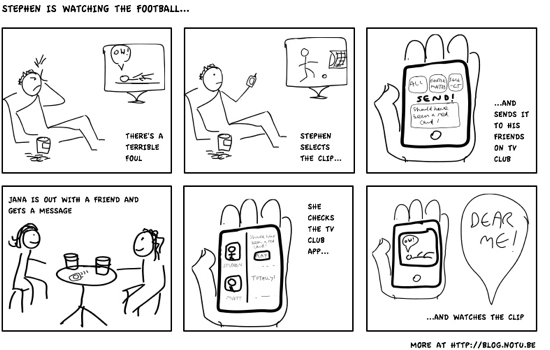
\includegraphics[width=6in]{images/postcard2.png}
\caption{A Possible Scenario} \label{fig:postcard2}
\end{center}
\end{figure}


\begin{figure}[htbp]
\begin{center}
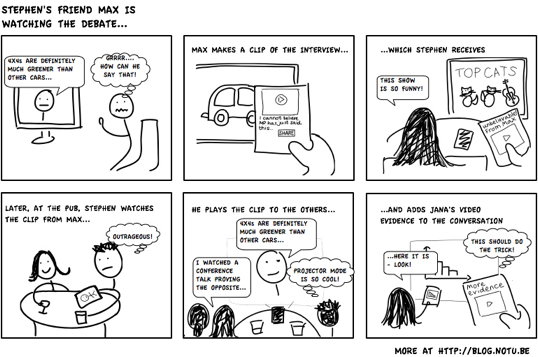
\includegraphics[width=6in]{images/postcard3.png}
\caption{A Possible Scenario} \label{fig:postcard3}
\end{center}
\end{figure}


\chapter{Conclusions}


Within this document we have justified our reasons for continuing to focus on second screens, APIs to TV and URLs for TV. We believe that one of the main strengths of this workpackage is in showing others what can be done in this area, using effective communication tools and techniques, such as the use of cartoon-strip style sketches to develop our ideas for realistic future scenarios. We made these into postcards\footnote{\url{http://www.flickr.com/photos/nicecupoftea/sets/72157624747199046/with/4902348004/}} to give away at IBC and other events, and these have generated a lot of interest. We have used opportunities to talk about our work in public, including the NoTube blog, and we have developed beneficial collaborative relationships with external parties such as Project Baird. By consolidating the infrastructure work from last year, we have also built three new prototypes which illustrate ways in which integrating `TV and the Social Web' can make the TV experience more enjoyable. We now have a clear plan for evaluation, and several research questions to consider.
 

\end{document}